\documentclass[conference]{IEEEtran}
\IEEEoverridecommandlockouts

\usepackage{cite}
\usepackage{amsmath,amssymb,amsfonts,amsthm}
\usepackage{algorithm}
\usepackage{algpseudocode}
\usepackage{graphicx}
\usepackage{textcomp}
\usepackage{xcolor}
\usepackage{booktabs}
\usepackage{url}
\usepackage[hidelinks]{hyperref}

% Definitions and remarks are set upright because they carry explanatory prose; claims that
% are proved (propositions) stay italic so they stand out from it.
\theoremstyle{plain}
\newtheorem{proposition}{Proposition}
\theoremstyle{definition}
\newtheorem{definition}{Definition}
\newtheorem{remark}{Remark}
\newtheorem{assumption}{Assumption}

\newcommand{\R}{\mathbb{R}}
\newcommand{\W}{\mathcal{W}}
\newcommand{\Obs}{\mathcal{O}}
\newcommand{\Rob}{\mathcal{R}}
\newcommand{\Cand}{\mathcal{C}}
\newcommand{\Bod}{\mathcal{B}}
\newcommand{\X}{\mathcal{X}}
\newcommand{\Uc}{\mathcal{U}}
\newcommand{\Core}{\mathcal{K}}
\newcommand{\clr}{\varepsilon}

\begin{document}

\title{Unsatisfiability as a Coordination Signal:\\
Core-Guided Trajectory Optimization for\\
Multi-Robot Kinodynamic Motion Planning}

% TODO: fill in the author block before submission. Square brackets must stay braced
% here -- a bare [ after \\ is parsed as the optional length argument of \\.
\author{\IEEEauthorblockN{{Author Name}}
\IEEEauthorblockA{\textit{{Department}} \\
\textit{{Institution}} \\
{City, Country} \\
{email@institution.edu}}
}

\maketitle

\begin{abstract}
Multi-robot kinodynamic planners resolve inter-robot conflicts reactively: a collision is
observed between two trajectories and that pair is re-planned. We keep the standard
machinery of such planners --- a geometric RRT guide per robot and a trajectory optimizer
that turns it into a dynamically feasible motion --- and change only what triggers
re-planning. Each robot owns a small, growing set of optimized candidate trajectories. A SAT
solver selects one candidate per robot, and pairwise collision clauses are added lazily, only
for the combinations the solver actually proposes. When the solver reports \textsc{unsat},
its \emph{unsatisfiable core} proves that the current candidates admit no collision-free
selection and names the refuted pairs responsible. Only those robots are re-optimized, each
from shortly before the contact the core names, keeping clear of the trajectory it collided
with. The same clause database then certifies the makespan: bisecting a horizon cap over the
candidates already built ends with a proof that no shorter selection exists among them. We
carry a four-robot instance through every step with the implementation's numbers (sixteen
optimizer calls, a round that proves a second impasse with no new collision checks, and a
certified makespan), and report first results on $16$- and $32$-robot scenarios, where a
reimplementation of K-ARC using the same trajectory optimizer does not solve the $32$-robot
Open Cross instance in any of five seeds.
\end{abstract}

\begin{IEEEkeywords}
multi-robot systems, kinodynamic motion planning, trajectory optimization, satisfiability
\end{IEEEkeywords}

\section{Introduction}

A multi-robot kinodynamic planner answers two questions of different kinds. The first is
continuous: what motion can one robot execute, given its acceleration limits, its turning
limits and the obstacles? The second is combinatorial: which motions do the robots execute
together, so that no two of them collide? Planners in this space, including K-ARC
\cite{karc2025}, db-CBS \cite{dbcbs2024} and db-LaCAM \cite{dblacam2025}, answer the second
question by repeatedly re-asking the first. A conflict between two trajectories is found,
a constraint is imposed, and the continuous planner is invoked again for that pair.

The signal that drives this loop is always of the form ``these two trajectories touch'',
which is a statement about one observed failure. A solver that reasons over a finite set of
candidate motions can return something strictly stronger when it fails: that \emph{no}
choice among the candidates works, together with the subset of known collisions that already
makes this impossible. Modern SAT solvers return exactly such a subset, the unsatisfiable
core, when asked to track which constraints they used \cite{z3}.

This paper uses that certificate as the trigger for re-planning and keeps everything else
standard. Each robot's motions come from a geometric RRT \cite{lavalle2001} refined by the
trajectory optimization program K-ARC uses \cite{karc2025}, built in CasADi
\cite{casadi2019} and solved with IPOPT \cite{ipopt2006}. We make no claim about either
component. The contribution is the loop around them: which robots are re-optimized, from
which moment, and against which trajectory, is decided by an unsatisfiable core rather than
by an observed collision, a priority order, or a random restart. Because the low-level solver
is identical to K-ARC's, a comparison against it measures the coordination alone.

\subsection*{Contributions}

\begin{enumerate}
  \item A formulation of multi-robot coordination as Boolean selection over per-robot sets of
        optimized trajectories, with collision clauses learned lazily and tracked so that
        failure yields a core (Sec.~\ref{sec:encoding}).
  \item A core-guided repair that re-optimizes each named robot from shortly before its
        named contact, keeping clear of the named trajectory, and offers both ways around
        (Sec.~\ref{sec:repair}).
  \item A makespan certificate obtained from the same clause database by horizon bisection
        (Prop.~\ref{prop:bisect}).
  \item A fully worked four-robot instance with the implementation's numbers
        (Sec.~\ref{sec:example}) and first results against K-ARC at $16$ and $32$ robots
        (Sec.~\ref{sec:experiments}).
\end{enumerate}

\section{Related Work}

Conflict-Based Search \cite{cbs2015} established the two-level pattern in which a low level
plans for one agent and a high level branches on an observed conflict between two agents.
db-CBS \cite{dbcbs2024} and db-LaCAM \cite{dblacam2025} carry the pattern into kinodynamic
settings by composing motion primitives, and K-ARC \cite{karc2025} builds a sub-problem
around each conflicting pair, solves it by trajectory optimization, and enlarges it when
resolving one conflict creates another. In all of these the unit of blame is a pair of
trajectories that were observed to touch. Prioritized planning \cite{erdmann1987} avoids
blame by fixing an order in advance.

Surynek \cite{surynek2020} gives the closest methodological precedent on the combinatorial
side: a lazy SMT encoding for continuous multi-agent path finding in which collision
constraints are added on demand. There the candidate structure is a fixed roadmap, so
unsatisfiability under a makespan bound is resolved by raising the bound. In our setting the
candidate sets themselves are refined, so unsatisfiability is a statement about the motions
generated so far, and the core says which of them to regenerate.

For continuous-time safety between polynomial trajectories, Park and Kim \cite{parkkim2020}
certify pairs through their relative Bernstein coefficients; we return to this in
Sec.~\ref{sec:properties}.

\section{Preliminaries}
\label{sec:prelim}

\begin{table}[t]
\caption{Notation.}
\label{tab:notation}
\centering
\small
\setlength{\tabcolsep}{3pt}
\begin{tabular}{@{}ll@{}}
\toprule
$\W,\ \Obs$ & workspace; static obstacles \\
$\Rob = \{0,\dots,N{-}1\}$ & robot indices \\
$q,\ u$ & state $(x,y,\theta,v,\omega)$; control $(a,\alpha)$ \\
$\Phi_i,\ \Delta t$ & one-step integrator of robot $i$; time step \\
$\tau_i,\ |\tau_i|$ & executed trajectory; its length in steps \\
$r^{+}_i,\ r^{-}_i$ & bounding, inscribed radius of the body \\
$d_{\text{surf}},\ \clr$ & surface distance; required clearance \\
$\kappa(\tau_i,\tau_j),\ \xi(\tau_i,\tau_j)$ & first contact step; first contact point \\
$\gamma_i$ & guide polyline from the RRT \\
$\textsc{Opt}$ & trajectory optimization (Def.~\ref{def:opt}) \\
$\Cand_i,\ \tau_i^{(c)}$ & candidate set of robot $i$; its $c$-th element \\
$x_{i,c},\ \ell_{i,c,j,c'}$ & selection variable; tracking literal \\
$\Core$ & unsatisfiable core \\
$g_i,\ \varrho,\ T_{\max}$ & goal; goal tolerance; horizon budget \\
$h$ & horizon cap used during bisection \\
\bottomrule
\end{tabular}
\end{table}

Table~\ref{tab:notation} collects the notation. Superscripts in parentheses, as in
$\tau_i^{(c)}$, index candidates; plain superscripts, as in $q_i^k$, index time steps.

\subsection{Workspace, robots and trajectories}
\label{sec:prelim-world}

\begin{definition}[Workspace, pose and occupancy]
The workspace $\W \subset \R^2$ is a bounded planar region --- a $17 \times 17$\,m square in
every instance of this paper --- containing a finite set $\Obs$ of static obstacles, each a
closed convex set. A pose $p = (x,y,\theta)$ places a robot at position $(x,y)$ facing
direction $\theta$. Robot $i$ has a rigid convex body $A_i$ described in its own frame, and
the region of the floor it covers at pose $p$ is
$\Bod_i(p) = \{\, R(\theta)\,z + (x,y)^{\!\top} : z \in A_i \,\}$, the body rotated by
$\theta$ and moved to $(x,y)$. Our robots are $0.5 \times 0.25$\,m boxes, for which heading
matters: the same box needs more room sideways than end-on.
\end{definition}

\begin{definition}[Second-order unicycle]
\label{def:robot}
Each robot follows the second-order unicycle with the parameters published for
\texttt{unicycle2\_v0} in dynobench \cite{dynobench}. Its state $q = (x,y,\theta,v,\omega)$
contains the pose together with the forward speed $v$ and turning rate $\omega$, and its
control $u = (a,\alpha)$ contains the corresponding accelerations:
\begin{equation}
  \dot x = v\cos\theta,\quad
  \dot y = v\sin\theta,\quad
  \dot\theta = \omega,\quad
  \dot v = a,\quad
  \dot\omega = \alpha .
  \label{eq:dyn}
\end{equation}
Because speeds are part of the state, the planner cannot change them instantaneously; it
chooses only how hard to accelerate and to start or stop turning. All quantities are bounded,
\begin{equation}
  |v| \le v_{\max},\quad |\omega| \le \omega_{\max},\quad
  |a| \le a_{\max},\quad |\alpha| \le \alpha_{\max},
  \label{eq:bounds}
\end{equation}
with $v_{\max}=0.5$\,m/s, $\omega_{\max}=0.5$\,rad/s, $a_{\max}=0.25$\,m/s$^2$ and
$\alpha_{\max}=0.25$\,rad/s$^2$. We write $\X$ and $\Uc$ for the states and controls
satisfying these bounds. A robot at full speed therefore needs $0.5$\,m to stop and cannot
turn tighter than a $1$\,m radius, both large compared with its body and with the $0.2$\,m
goal tolerance.
\end{definition}

\begin{definition}[Executed trajectory]
\label{def:exec}
Time advances in steps of $\Delta t = 0.1$\,s. The map $\Phi_i : \X \times \Uc \to \X$
advances robot $i$ by one step, integrating \eqref{eq:dyn} with fourth-order Runge--Kutta and
saturating $v$ and $\omega$ to their bounds. Applying controls
$u_i^0,\dots,u_i^{T-1} \in \Uc$ one after another from a start state $q_i^0$ produces the
executed trajectory $\tau_i = (q_i^1,\dots,q_i^T)$ with $q_i^{k+1} = \Phi_i(q_i^k,u_i^k)$,
whose length $|\tau_i| = T$ is its duration in steps. Everything the planner checks and
reports is defined on $\tau_i$ produced this way, which is the same integrator the simulator
executes.
\end{definition}

\subsection{Collision semantics}
\label{sec:prelim-collision}

\begin{definition}[Surface distance and radii]
The surface distance
$d_{\text{surf}}(i,p,\,j,p') = \min\{\lVert z - z'\rVert : z \in \Bod_i(p),\ z' \in
\Bod_j(p')\}$ is the length of the shortest gap between two bodies' outlines; it is zero
exactly when they touch or overlap, and for boxes it is computed exactly. The bounding radius
$r^{+}_i$ is the radius of the smallest disc around the body's centre that contains it
whatever its heading, and the inscribed radius $r^{-}_i$ that of the largest disc it
contains. For our robots $r^{+} = 0.2795$\,m and $r^{-} = 0.125$\,m.
\end{definition}

\begin{proposition}[Three-band test]
\label{prop:bands}
For two robots whose centres are $\delta$ apart and a clearance $\clr \ge 0$,
$\delta \ge r^{+}_i + r^{+}_j + \clr$ implies $d_{\text{surf}} \ge \clr$, and
$\delta < r^{-}_i + r^{-}_j + \clr$ implies $d_{\text{surf}} < \clr$.
\end{proposition}

\begin{proof}
Each body lies inside its bounding disc and contains its inscribed disc, so
$\delta - r^{+}_i - r^{+}_j \le d_{\text{surf}} \le \delta - r^{-}_i - r^{-}_j$.
\end{proof}

Only centre distances between the two sums need the exact box distance. For our robots and
$\clr = 0.05$\,m that is the ring $0.300 \le \delta < 0.609$\,m; most steps of most pairs are
farther apart, and a centre distance is one subtraction.

\begin{definition}[Conflict and first contact]
\label{def:conflict}
Two executed trajectories $\tau_i,\tau_j$ conflict when, at some step $k$,
$d_{\text{surf}}(i,p_i^k,\,j,p_j^k) < \clr$. Both are compared on a common clock, and the
shorter one is held at its final state beyond its own length, since a robot that has arrived
still occupies its goal. The first such step is the \emph{first contact step}
$\kappa(\tau_i,\tau_j)$, and the midpoint of the two centres at that step is the \emph{first
contact point} $\xi(\tau_i,\tau_j)$. If no step conflicts we write $\kappa = \xi = \bot$. The
point answers where the two robots met and the step answers when; the repair of
Sec.~\ref{sec:repair} uses both.
\end{definition}

\subsection{Guides and trajectory optimization}
\label{sec:prelim-opt}

\begin{definition}[Guide]
\label{def:guide}
A guide $\gamma_i$ is a collision-free polyline from robot $i$'s start to its goal, produced
by a rapidly-exploring random tree \cite{lavalle2001} for a disc of radius $r^{+}_i + \clr$
--- the disc that covers the robot at any heading, plus clearance --- followed by random
shortcutting, which repeatedly replaces a stretch of the path by a straight segment whenever
that segment is also collision-free. The tree grows in steps of $0.6$\,m and aims at the goal
one draw in ten. A guide carries no timing and no dynamics; it only says which way around the
obstacles to go.
\end{definition}

\begin{definition}[Trajectory optimization]
\label{def:opt}
The call $\textsc{Opt}(i, q, n, \gamma, \tau')$ solves, for robot $i$, a nonlinear program
over $n$ steps of length $\Delta t$ with decision variables $q^0,\dots,q^n$ and
$u^0,\dots,u^{n-1}$:
\begin{equation}
\begin{aligned}
  \min_{q,u}\ & \textstyle \beta \sum_{k} \lVert u^k \rVert^2 \\
  \text{s.t.}\ & q^0 = q, \quad q^{k+1} = \mathrm{RK4}(q^k, u^k, \Delta t), \\
  & q^k \in \X,\ u^k \in \Uc,\ \text{centre at least } r^{+}_i \text{ inside } \W, \\
  & \operatorname{dist}\!\big((x^k,y^k), o\big) \ge r^{+}_i + \clr \quad
    \forall o \in \Obs \text{ near } \gamma, \\
  & \lVert (x^n,y^n) - g_i \rVert \le 0.15, \quad v^n = \omega^n = 0, \\
  & \textsc{Clear}(q^k, \tau'^{\,k}) \quad \text{for every } k \text{ (if } \tau' \text{ given)}.
\end{aligned}
\label{eq:opt}
\end{equation}
The dynamics are enforced at every step with the same Runge--Kutta rule the simulator uses,
so a converged solution is, up to solver tolerance, a trajectory the robot really executes.
The robot must stay inside the workspace, keep its bounding disc plus clearance away from
every obstacle within $4$\,m of the guide, and come to rest within $0.15$\,m of its goal after
exactly $n$ steps. The objective penalises control effort with $\beta = 0.01$; with the step
length fixed, the duration is chosen by the caller through $n$, not by the solver. The initial
iterate places the positions along $\gamma$ at equal arclength and the heading along the
guide's direction, which matters because a nonlinear program does not change which side of an
obstacle it passes during a solve. Finally, $\tau'$ is an optional trajectory of another robot
to keep clear of: $\textsc{Clear}$ covers each body by three discs of radius $0.150$\,m spaced
along its long axis and requires every disc of one robot to stay $2 \cdot 0.150 + \clr =
0.350$\,m from every disc of the other at the same step, which contains the true bodies and
so is conservative. This is K-ARC's program \cite{karc2025} with the step length fixed to the
simulator's instead of left free, built in CasADi
\cite{casadi2019} and solved by IPOPT \cite{ipopt2006}. A call either converges or fails, and
only converged solutions are used.
\end{definition}

Two simple durations recur. Along a guide of length $L$, a robot that accelerates at
$a_{\max}$ to $v_{\max}$, cruises and brakes needs
\begin{equation}
  n_{\text{bb}}(L) = \left\lceil \big(L/v_{\max} + v_{\max}/a_{\max}\big)/\Delta t \right\rceil
  \label{eq:nbb}
\end{equation}
steps, which is $320$ steps for the $15$\,m crossings of our instances. Candidates are
requested with durations that are multiples of this figure.

\subsection{Satisfiability and cores}
\label{sec:prelim-sat}

A SAT solver receives Boolean variables and logical constraints over them, and either returns
an assignment satisfying all constraints or proves that none exists. We use z3 \cite{z3},
which also accepts cardinality constraints such as ``exactly one of these variables is
true'' directly.

\begin{definition}[Tracked constraint and unsatisfiable core]
\label{def:core}
A constraint $\phi$ is tracked by attaching a fresh literal $\ell$ that the solver assumes
true, asserting $\ell \rightarrow \phi$. When the constraints are unsatisfiable, the solver
returns an unsatisfiable core $\Core$: a set of tracking literals whose constraints are
already contradictory on their own, together with the untracked ones. The literals act as
name tags, and the core is the list of names the solver needed to prove impossibility. It is
a sufficient explanation rather than a guaranteed minimal one, but every constraint it names
is one that was actually asserted.
\end{definition}

\begin{definition}[Lazy refinement]
\label{def:cegar}
A constraint too large to write out in full is added lazily: the solver proposes an
assignment without it, an \emph{oracle} tests the proposal, and each failure the oracle finds
is returned to the solver as a new constraint forbidding it. The loop stops when the oracle
accepts a proposal or the solver proves that none remains. This is counterexample-guided
abstraction refinement, used for continuous multi-agent path finding in \cite{surynek2020}.
Here the constraint too large to write out is ``no two chosen trajectories collide'', and the
oracle is Def.~\ref{def:conflict}.
\end{definition}

\section{Problem Statement}
\label{sec:problem}

An instance consists of the workspace and obstacles, the robots $\Rob$ with their bodies,
start states $q_i^0$ at rest and goal positions $g_i$, the time step $\Delta t$, a horizon
budget $T_{\max}$, the required clearance $\clr = 0.05$\,m, and a goal tolerance
$\varrho = 0.2$\,m.

\begin{definition}[Admissible plan]
\label{def:plan}
A plan assigns each robot a control sequence; sequences are padded with zero controls to a
common length $T$ so that finished robots stay at rest, and they induce executed trajectories
$\tau_i$ by Def.~\ref{def:exec}. The plan is admissible when
(P1) every control lies in $\Uc$;
(P2) no body intersects an obstacle at any step $k \le T$;
(P3) every pair of robots keeps $d_{\text{surf}} \ge \clr$ at every step $k \le T$;
(P4) every robot ends within $\varrho$ of its goal; and
(P5) $T \le T_{\max}$.
The problem is to find an admissible plan with a small makespan $T\Delta t$, the time at which
the last robot finishes, or to report failure.
\end{definition}

Conditions (P2) and (P3) are required at the time steps, which is the semantics under which
the simulator scores collisions; Remark~\ref{rem:gap} states what this leaves open between
steps. For clarity all robots share one model and one body, but every bound is read per robot
and Def.~\ref{def:conflict} is already per pair, so heterogeneous teams need no change to the
method.

\section{Method}
\label{sec:method}

\subsection{Overview}

Each robot $i$ keeps a candidate set $\Cand_i = \{\tau_i^{(0)}, \tau_i^{(1)}, \dots\}$ of
executed trajectories from its start to its goal, each produced by $\textsc{Opt}$ for that
robot alone. The set only grows. Coordination is the discrete choice of one candidate per
robot such that no two chosen candidates conflict, and one round of the method proceeds as
follows. The solver proposes a choice subject to every collision learned so far; the oracle
checks the proposal pair by pair and returns each collision it finds as a new constraint,
until the solver either produces a collision-free choice or proves that none exists. In the
first case the choice is verified and shortened by bisection. In the second, the core names
the refuted pairs the proof needed, and each robot in them receives new candidates that
re-optimize its trajectory around the contact. Algorithm~\ref{alg:main} states the loop.

\begin{algorithm}[t]
\caption{Core-guided coordination}
\label{alg:main}
\begin{algorithmic}[1]
\Require instance, round cap $N_r$, deadline $D$
\Ensure an admissible plan, or \textsc{fail}
\For{$i \in \Rob$}
  \State $\gamma_i \gets \textsc{Guide}(i)$;\quad $n \gets n_{\text{bb}}(\text{length of } \gamma_i)$
  \State $\Cand_i \gets \{\textsc{Opt}(i, q_i^0, \lceil 1.3n \rceil, \gamma_i),\
                          \textsc{Opt}(i, q_i^0, \lceil 1.6n \rceil, \gamma_i)\}$
\EndFor
\State $\Gamma \gets \emptyset$ \Comment{learned collisions, never retracted}
\For{$r = 1 \dots N_r$}
  \State $(\pi, \text{verdict}, \Core) \gets \textsc{Search}(\Cand, \Gamma, h=\infty)$
  \State \textbf{if} verdict $=$ \textsc{timeout} \textbf{then return} \textsc{fail}
  \State \textbf{if} verdict $=$ \textsc{sat} \textbf{then return} $\textsc{Bisect}(\pi, \Cand, \Gamma)$
  \State $\textsc{Repair}(\Cand, \Core)$ \Comment{Alg.~\ref{alg:repair}}
\EndFor
\State \Return \textsc{fail}
\Statex
\Function{Search}{$\Cand, \Gamma, h$}
  \State assert $\sum_{c} x_{i,c} = 1$ for each $i$; forbid $x_{i,c}$ if $|\tau_i^{(c)}| > h$
  \State assert every clause of $\Gamma$, tracked
  \While{true}
    \State \textbf{if} $\textsc{now}() > D$ \textbf{then return} $(\bot, \textsc{timeout}, \emptyset)$
    \State \textbf{if} $\textsc{check}() = \textsc{unsat}$ \textbf{then return} $(\bot, \textsc{unsat}, \textsc{core}())$
    \State $\pi \gets$ one candidate index $\pi_i$ per robot
    \State $F \gets \{(i,j) : i<j,\ \kappa(\tau_i^{(\pi_i)}, \tau_j^{(\pi_j)}) \neq \bot\}$
    \If{$F = \emptyset$}
      \State \textbf{if} \textsc{Verify}$(\pi)$ \textbf{then return} $(\pi,\textsc{sat},\emptyset)$
      \State assert $\bigvee_i \neg x_{i,\pi_i}$ \Comment{untracked}
    \Else
      \State add $\ell_{i,\pi_i,j,\pi_j} \rightarrow (\neg x_{i,\pi_i} \vee \neg x_{j,\pi_j})$
             to $\Gamma$ for each $(i,j) \in F$
    \EndIf
  \EndWhile
\EndFunction
\end{algorithmic}
\end{algorithm}

\subsection{Seeding}
\label{sec:seeding}

Every robot starts with one guide (Def.~\ref{def:guide}) and two candidates obtained from
it: a fast one with $\lceil 1.3\, n_{\text{bb}} \rceil$ steps and a slow one with
$\lceil 1.6\, n_{\text{bb}} \rceil$ steps, where $n_{\text{bb}}$ is \eqref{eq:nbb} for the
guide's length. The factor leaves room for the optimizer: on a cluttered $17$\,m crossing a
duration of exactly $n_{\text{bb}}$ failed to converge where $1.3\,n_{\text{bb}}$ succeeded. The slow candidate gives the solver a way to let another robot pass first without
any geometric change. Each converged solution is re-driven from the robot's start through
$\Phi_i$ with its controls clipped into $\Uc$, and it is this executed trajectory, not the
solver's iterate, that enters $\Cand_i$. All calls within a batch are independent and run in
parallel worker processes.

\subsection{Boolean encoding}
\label{sec:encoding}

For each robot $i$ and candidate index $c$ a Boolean variable $x_{i,c}$ states that robot $i$
executes its $c$-th candidate. The formula has three parts. An exactly-one constraint per
robot,
\begin{equation}
  \textstyle\sum_{c\,:\,|\tau_i^{(c)}| \le h} x_{i,c} = 1,
  \qquad x_{i,c} = \text{false whenever } |\tau_i^{(c)}| > h,
  \label{eq:exactlyone}
\end{equation}
makes every robot pick exactly one candidate no longer than the horizon cap $h$, which is
unbounded during the rounds and is lowered during bisection. For every pair of candidates the
oracle has refuted --- robot $i$ on candidate $c$ against robot $j$ on candidate $c'$ --- the
clause
\begin{equation}
  \ell_{i,c,j,c'} \rightarrow \big(\neg x_{i,c} \vee \neg x_{j,c'}\big)
  \label{eq:clause}
\end{equation}
says that the two robots may not both take those candidates, and its tracking literal
$\ell_{i,c,j,c'}$ lets a core name it. Finally, when a choice passes every pairwise check but
fails the full verifier of Sec.~\ref{sec:verify}, an untracked clause forbids that exact
choice. No variable stands for a time, a position or a speed; all continuous content lives in
the candidates, so the solver's problem stays small however long the trajectories are.

\subsection{The oracle and the cache}
\label{sec:oracle}

The oracle evaluates Def.~\ref{def:conflict} with Prop.~\ref{prop:bands}, computing all centre
distances of a pair at once and reaching the exact box distance only in the ring between the
two radii. Every refutation is cached with its contact point and re-asserted in every later
solver call, so a pair of candidates is checked at most once over the whole run, and a
collision learned in one round constrains every later round and every bisection probe.

\subsection{Core-guided repair}
\label{sec:repair}

When the solver proves that no choice exists, it returns a core $\Core$ of tracking literals.
Each literal $\ell_{i,c,j,c'}$ names a refuted pair: robot $i$ on candidate $c$ met robot $j$
on candidate $c'$. The robots appearing in $\Core$ are exactly those the proof needed, and the
refuted pairs say whom they met, on which candidates, and when. Repair acts on this
information and on nothing else (Algorithm~\ref{alg:repair}).

\begin{algorithm}[t]
\caption{\textsc{Repair}: yield candidates from a core}
\label{alg:repair}
\begin{algorithmic}[1]
\Require candidate sets $\Cand$, core $\Core$, start offset $w=30$ steps
\For{each robot $i$ named in $\Core$, with its first literal $\ell_{i,c,j,c'}$}
  \State $\tau \gets \tau_i^{(c)}$;\quad $\tau' \gets \tau_j^{(c')}$;\quad $k \gets \kappa(\tau, \tau')$
  \For{$w' \in \{w, 2w, 4w\}$}
    \State $s \gets \max(k - w', 0)$;\quad $n \gets \lceil 1.2\,(|\tau| - s) \rceil$
    \For{$\sigma \in \{+1, -1\}$}
      \State $\hat\gamma \gets$ remainder of $\tau$ after step $s$, pushed $0.9\sigma$\,m aside at step $k$
      \State $\tau^\ast \gets \textsc{Opt}(i, q^s(\tau), n, \hat\gamma, \tau' \text{ from step } s)$
      \State \textbf{if} converged \textbf{then} add (first $s$ steps of $\tau$) $\oplus\ \tau^\ast$ to $\Cand_i$
    \EndFor
    \State \textbf{if} any side converged \textbf{then break}
  \EndFor
\EndFor
\end{algorithmic}
\end{algorithm}

For a robot $i$ named by a refuted pair, the repair keeps its candidate $\tau$ unchanged up
to $s$ steps, where $s$ lies $w = 30$ steps ($3$\,s) before the first contact step $k$, and
re-optimizes the rest of the motion from the state reached at step $s$ to the goal while
keeping clear of the other robot's candidate $\tau'$ from step $s$ onwards. The robot thus
learns to step aside for precisely the trajectory it collided with, starting from precisely
the moment the collision became imminent. The new candidate is the unchanged prefix followed
by the re-optimized remainder, re-driven through $\Phi_i$ from the start.

Three choices in this step are forced by the dynamics rather than taken for convenience. The
re-optimized stretch runs to the goal rather than rejoining the old trajectory at a fixed later
step: a robot at cruise speed has no spare time, a sidestep is longer than the stretch it
replaces, and in our measurements every re-optimization of a $6$\,s or $12$\,s window with both
ends fixed failed to converge. The remainder is given $20\%$ more steps than it had,
$n = \lceil 1.2\,(|\tau| - s)\rceil$, because with no extra time the sidestep again failed in
every case we tried. The initial iterate is the old remainder pushed $0.9$\,m sideways around
the contact step, with a smooth bump that is zero at step $s$ and again after $2(k-s)$ steps,
and both sides are tried: the core says where two robots meet but not which way round, and one
side may be a wall --- with the initial iterate pushed into the workspace boundary, every
re-optimization of our head-on test pair failed, and with it pushed the other way every one
converged. If neither side converges, the offset doubles to $6$\,s and
then $12$\,s. Both robots of a refuted pair are repaired, each yielding to the other, and the
solver later decides which of the two actually yields. If the core contains no tracked literal
at all, every robot receives a fresh guide and fresh fast and slow candidates.

\begin{remark}[What the core adds over a pairwise conflict]
\label{rem:corevspair}
A pairwise conflict says that two trajectories touch. The core says that no choice among all
candidates is collision-free and that the named collisions already prove it. Repair therefore
runs only after every alternative already present --- every combination of fast, slow and
earlier yield candidates --- has been ruled out by the solver without any new optimization.
Robots not in the core are left alone even if their current candidates also collide with
something, because the proof did not need them. And since candidate sets only grow and clauses
are never retracted, nothing proved in an earlier round has to be proved again.
\end{remark}

\subsection{Verification}
\label{sec:verify}

Before a choice is accepted, its candidates are padded to a common length by holding each
robot at its final state, and the padded plan is checked against Def.~\ref{def:plan} by the
simulator's own collision routine: every pair and every obstacle at every step, goal arrival
and the horizon budget. A choice that survives the pairwise checks can still fail here, and is
then forbidden by an untracked clause.

\subsection{Horizon bisection}
\label{sec:bisect}

The first admissible choice is rarely the shortest, since the cheapest way out of a conflict
is often a slower candidate. With $T^\ast$ the length of the best plan so far and
$T_{\text{lo}} = \max_i \min_c |\tau_i^{(c)}|$ --- no plan can finish before every robot's
shortest candidate does --- the method repeats, for at most $12$ probes and while
$T_{\text{lo}} < T^\ast$, a search with horizon cap
$h = \lfloor (T_{\text{lo}} + T^\ast - 1)/2 \rfloor$. A plan found under the cap replaces the
best plan; a proof of impossibility raises $T_{\text{lo}}$ to $h + 1$. No optimization is
performed during bisection and every cached collision is reused, so probes cost solver time
and the occasional pairwise check.

\begin{proposition}[Makespan certificate]
\label{prop:bisect}
If bisection stops because $T_{\text{lo}} \ge T^\ast$, no choice from the final candidate sets
that finishes within $T^\ast - 1$ steps passes both the pairwise oracle and the verifier; the
returned plan is makespan-optimal over the candidates that were built.
\end{proposition}

\begin{proof}
$T_{\text{lo}}$ is raised to $h+1$ only when the search under cap $h$ is unsatisfiable. Every
clause forbids either a pair the oracle refuted or a choice the verifier rejected, so no
choice within that cap passes both, and the same holds for every smaller cap. Candidate sets
do not change during bisection, and the initial $T_{\text{lo}}$ is a valid lower bound.
\end{proof}

The proposition concerns the candidates, not all possible motions: a shorter plan may exist
using trajectories the method never generated. It does turn the shortest plan the method
happened to find into the shortest plan its candidates allow, proved by the same machinery
that proved the impasses.

\subsection{Budget}

A single wall-clock deadline is checked before every solver call. Optimizer batches and
single solver calls are not interrupted, so a run can overrun its deadline by the length of
one batch.

\section{Properties}
\label{sec:properties}

\begin{proposition}[Soundness in discrete time]
\label{prop:sound}
Every plan returned by Algorithm~\ref{alg:main} satisfies (P1)--(P5).
\end{proposition}

\begin{proof}
Every candidate is the result of driving clipped controls through $\Phi_i$, which gives
(P1), and padding adds zero controls. (P2)--(P5) are checked on the padded executed
trajectories by the verifier, which is the predicate the simulator scores with, and a plan
failing any of them is not returned.
\end{proof}

The optimization in \eqref{eq:opt} already imposes obstacle clearance, goal arrival and the
dynamics, so the verifier rarely rejects; it is there because the optimizer's obstacle model
is a disc, obstacles far from the guide are omitted from the program, and convergence is up
to a numerical tolerance. In our runs the re-driven trajectories coincided with the
optimizer's states to four decimal places.

\begin{proposition}[Monotonicity]
\label{prop:monotone}
Across rounds and bisection probes the clause set and every candidate set only grow; a pair
refuted once is refuted in every later solver call.
\end{proposition}

\begin{proof}
Repair appends candidates under new indices and never modifies an existing one, and a clause
refers to fixed indices whose trajectories never change.
\end{proof}

The method is not complete. It is complete relative to its candidates, in the sense that an
unsatisfiable verdict is a genuine proof that the candidates built so far cannot be combined,
but guides are random, rounds are capped, and the deadline is wall-clock. What the core
guarantees is that new optimization happens only once the old candidates have been proved
insufficient, and only for the robots that proof involves.

\begin{remark}[The gap between steps]
\label{rem:gap}
Prop.~\ref{prop:sound} holds at the time steps. Between two steps a pair's relative position
changes by at most $(v_i + v_j)\Delta t = 0.10$\,m, while the tightest passes in our plans
leave as little as $0.051$\,m. Inflating $\clr$ by $(v_i + v_j)\Delta t/2$ would close the
gap conservatively; certifying each interval exactly, as \cite{parkkim2020} do for polynomial
trajectories, would close it tightly. We state the gap rather than claim a continuous-time
guarantee.
\end{remark}

\section{A Fully Worked Instance}
\label{sec:example}

\begin{figure*}[p]
\centering
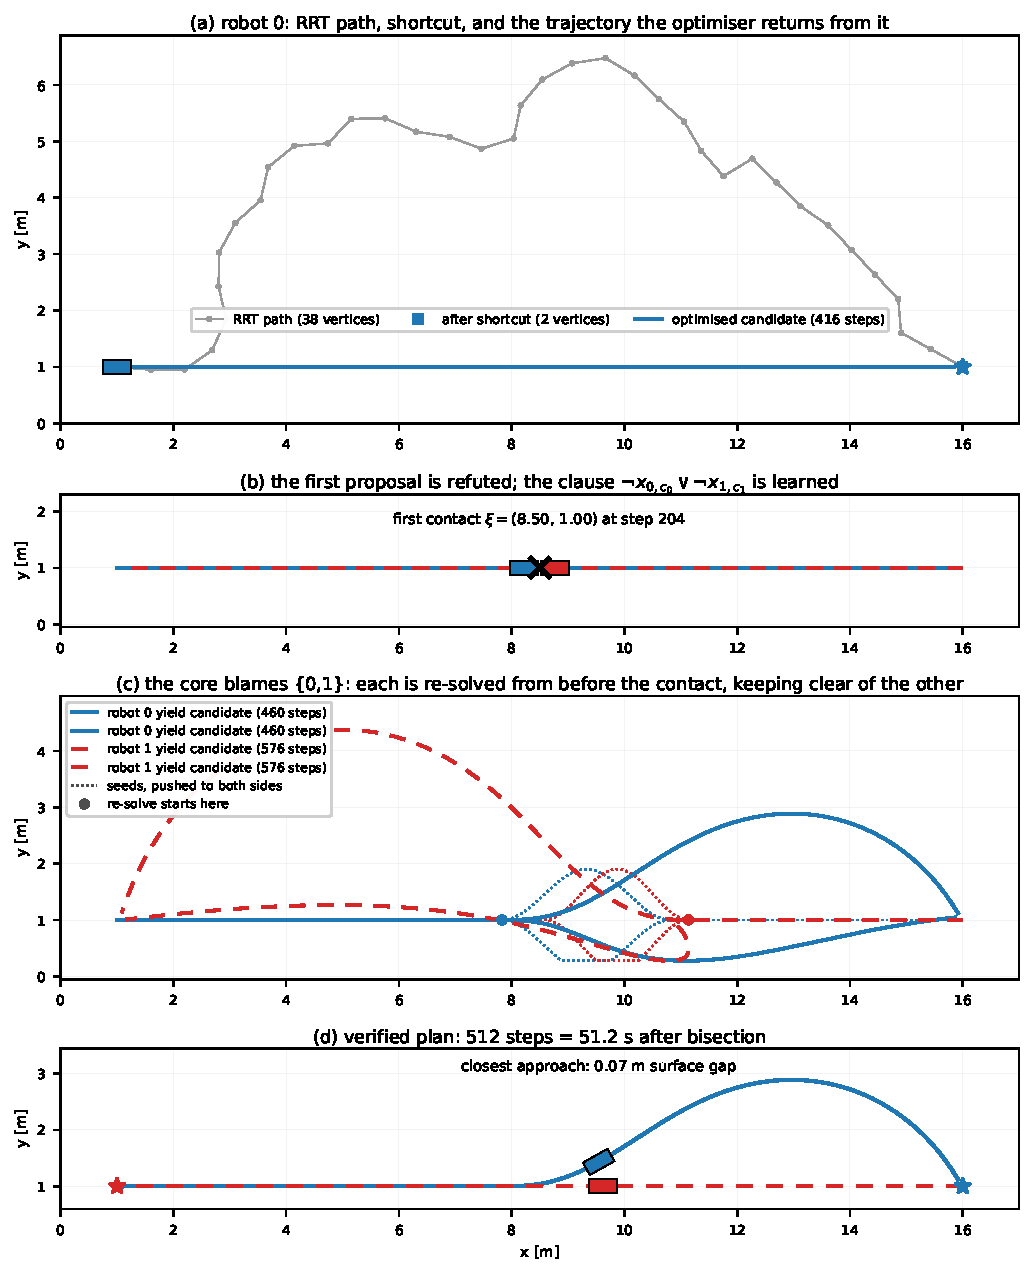
\includegraphics[width=0.86\textwidth]{figs/worked_example_trajopt.pdf}
\caption{The loop on the lower row of \texttt{open\_cross\_4}. Robot $0$ is blue and solid,
robot $1$ red and dashed; starts are drawn as bodies and goals as stars, and every panel is to
scale.
\textbf{(a)} Robot $0$'s guide: the raw RRT path ($38$ vertices, grey) shortcuts to a single
segment, and the optimizer turns it into the fast candidate of $416$ steps.
\textbf{(b)} The first proposal pairs the two fast candidates, which meet at
$\xi = (8.50, 1.00)$ at step $204$; the clause forbidding that pair is learned.
\textbf{(c)} In round $2$ the core names this row. Each robot is re-optimized from $3$\,s before
its contact (dots) with initial iterates pushed to both sides (dotted), keeping clear of the
other robot's candidate; all four calls converge.
\textbf{(d)} The verified plan: robot $1$ drives straight on its slow candidate while robot $0$
takes its yield candidate around it, passing at $0.07$\,m of surface clearance; $512$ steps,
certified minimal over the candidates by bisection.}
\label{fig:worked}
\end{figure*}

This section runs the method once on a small instance and reports the numbers that run
produced.

\subsection{The instance}

The instance is \texttt{open\_cross\_4}, a four-robot port of K-ARC's Open Cross benchmark
\cite{karc2025}, in which the robots of each row swap ends across an empty room. Robots $0$
and $1$ start at $(1,1)$ and $(16,1)$ facing each other and swap; robots $2$ and $3$ do the
same at $y = 16$. Each crossing is $15$\,m, the budget is $T_{\max} = 1300$ steps, the goal
tolerance $\varrho = 0.2$\,m, the clearance $\clr = 0.05$\,m, and the planner seed is $0$. The
two rows are $15$\,m apart and can never interact, so the correct blame is $\{0,1\}$ or
$\{2,3\}$ but never a mixture, which lets us check whether the core finds it.

\subsection{Seeding}

In an empty room the RRT still wanders: robot $0$'s raw path has $38$ vertices and climbs to
$y \approx 6.5$\,m before returning (Fig.~\ref{fig:worked}(a)). Shortcutting reduces it to the
straight $15$\,m segment from start to goal, and the same happens for every robot. With
$n_{\text{bb}} = 320$ steps, each robot receives a fast candidate of $416$ steps and a slow one
of $512$ steps. Both run straight, deviating by at most $6$\,mm; the fast one reaches the full
$0.5$\,m/s and the slow one peaks at $0.435$\,m/s. They stop $0.15$\,m short of the goal, the
optimizer's terminal tolerance. All eight calls converge, so $|\Cand| = (2,2,2,2)$.

\subsection{Round 1: refute, prove, explain, repair}

The solver's first proposal is refuted on both rows: robots $0$ and $1$ meet at
$\xi = (8.50,\,1.00)$ at step $204$, and robots $2$ and $3$ at $(8.50,\,16.00)$
(Fig.~\ref{fig:worked}(b)). The solver keeps proposing and the oracle keeps refuting, until all
$2 \times 2$ combinations within each row have been refuted: $8$ refutations after $24$ pairwise
checks, the other $16$ checks being between rows and clear. Slowing one robot moves the meeting
point along the row but does not remove it, and the solver reports that no choice exists.

This is where the method departs from a conflict-driven planner. The solver has ruled out every
combination of fast and slow candidates before any new optimization is requested, and its core
names the upper row. Robots $2$ and $3$ are each re-optimized from step $174$, $30$ steps
before their contact at step $204$, with $\lceil 1.2 \cdot (416-174) \rceil = 291$ remaining
steps, keeping clear of the other's candidate. All four calls converge. Each robot obtains two
yield candidates of $465$ steps: one sidesteps by $0.72$\,m towards the nearby wall, which is as
far as the workspace bound allows, and the other swings $2.17$\,m the other way. Now
$|\Cand| = (2,2,4,4)$.

\subsection{Round 2: the same proof, for free}

Round $2$ performs no new pairwise checks. The upper row can now be satisfied, but the lower
row is still ruled out entirely by the four clauses cached in round $1$, and the solver reports
impossibility at once. This time the core names robot $0$'s fast candidate against robot $1$'s
slow one, which meet right of centre, at $(9.60,\,1.00)$ and step $226$, because robot $1$ is
slower. Robot $0$ is re-optimized from step $196$ with $\lceil 1.2 \cdot (416 - 196)\rceil = 264$
remaining steps, and robot $1$ from the same step with $\lceil 1.2 \cdot (512-196) \rceil = 380$,
each keeping clear of the other's named candidate (Fig.~\ref{fig:worked}(c)). All four calls
converge, giving robot $0$ yield candidates of $460$ steps and robot $1$ yield candidates of
$576$ steps, so $|\Cand| = (4,4,4,4)$ after sixteen optimizer calls in total, none of which
failed. Prop.~\ref{prop:monotone} is visible here: the geometric work of round $1$ sufficed, on
its own, to prove the second impasse.

\subsection{Round 3: satisfy, verify, shorten}

Round $3$ needs $12$ more pairwise checks and finds one more refutation, at
$(8.50,\,1.01)$, before the solver proposes a choice that passes every check and the verifier:
robots $0$ and $2$ take yield candidates and robots $1$ and $3$ their slow ones, for $T = 512$
steps.

Bisection starts from $T^\ast = 512$ and $T_{\text{lo}} = 416$ and probes the caps $463$, $487$,
$499$, $505$, $508$, $510$ and $511$, each of which is proved impossible; the probe at $487$
learns one further refutation along the way. Bisection therefore stops with
$T_{\text{lo}} = T^\ast = 512$, and Prop.~\ref{prop:bisect} certifies that no choice among these
$16$ candidates finishes sooner. The reason is visible in the candidate lengths. Under any cap
below $512$, robot $1$ is left with only its fast candidate, since its slow and yield candidates
take $512$ and $576$ steps. Robot $0$'s fast candidate collides with it, and robot $0$'s yield
candidates were optimized to keep clear of robot $1$'s \emph{slow} candidate, the one named by
the core, not of the fast one --- which is exactly the refutation learned at $487$. The
makespan is set by that one choice of partner.

The returned plan is shown in Fig.~\ref{fig:worked}(d) and Table~\ref{tab:result}. In each row
one robot drives straight on its slow candidate while the other takes a yield candidate around
it at full speed. Which robot yields is chosen by the solver; the method contains no priority
rule. Table~\ref{tab:rounds} summarises the run.

\begin{table}[t]
\caption{The returned plan. Excursion is the largest distance from the straight line between
start and goal; arrival is the first time within $\varrho$ of the goal.}
\label{tab:result}
\centering
\small
\setlength{\tabcolsep}{4pt}
\begin{tabular}{lcrrrrr}
\toprule
robot & cand. & excursion & arrival & path & $\max|v|$ & $\max|\omega|$ \\
      &       & [m] & [s] & [m] & [m/s] & [rad/s] \\
\midrule
$0$ & yield & $1.889$ & $44.4$ & $16.00$ & $0.500$ & $0.192$ \\
$1$ & slow  & $0.006$ & $49.4$ & $14.85$ & $0.435$ & $0.000$ \\
$2$ & yield & $2.167$ & $44.9$ & $16.14$ & $0.500$ & $0.194$ \\
$3$ & slow  & $0.006$ & $49.4$ & $14.85$ & $0.435$ & $0.000$ \\
\midrule
\multicolumn{7}{l}{makespan $51.2$\,s ($512$ steps), verified by the simulator's checker}\\
\multicolumn{7}{l}{closest pass: pair $(0,1)$ $0.072$\,m at step $232$; pair $(2,3)$ $0.676$\,m}\\
\bottomrule
\end{tabular}
\end{table}

\begin{table}[t]
\caption{Round-by-round trace. Checks and refutations are cumulative; round~2 performs no new
checks.}
\label{tab:rounds}
\centering
\small
\setlength{\tabcolsep}{4pt}
\begin{tabular}{crrcll}
\toprule
rnd & checks & refut. & core names & new calls & $|\Cand|$ \\
\midrule
$0$ & ---  & --- & ---       & $8$ & $(2,2,2,2)$ \\
$1$ & $24$ & $8$ & $\{2,3\}$ & $4$ & $(2,2,4,4)$ \\
$2$ & $24$ & $8$ & $\{0,1\}$ & $4$ & $(4,4,4,4)$ \\
$3$ & $36$ & $9$ & ---       & $0$ & $T = 512$, certified \\
\bottomrule
\end{tabular}
\end{table}

\section{Experimental Evaluation}
\label{sec:experiments}

We use ports of K-ARC's Open Cross and Cluttered Cross scenarios \cite{karc2025}. The ports
follow the published description, which gives no workspace size, clearance, time step or
velocity limits, so ours are the values of Sec.~\ref{sec:example} and Def.~\ref{def:robot}. A
run succeeds only if its plan, executed in the simulator, reaches every goal with zero
collisions. The baseline is our reimplementation of K-ARC using the same trajectory optimizer,
with bodies covered by three discs as in \eqref{eq:opt} and a $1800$\,s budget; our method has a
$600$\,s budget and four optimizer processes. Wall times are Python on one shared machine and
not comparable to published C++ numbers.

\begin{table}[t]
\caption{First results. Ours: one seed per scenario. K-ARC: five seeds, same optimizer.
\texttt{open\_16} abbreviates \texttt{open\_cross\_16}, etc.}
\label{tab:results}
\centering
\small
\setlength{\tabcolsep}{3pt}
\begin{tabular}{lcccc}
\toprule
 & \multicolumn{2}{c}{ours (seed $0$)} & \multicolumn{2}{c}{K-ARC (5 seeds)} \\
\cmidrule(lr){2-3}\cmidrule(l){4-5}
scenario & plan & wall [s] & succ. & wall [s] \\
\midrule
\texttt{open\_16}      & ---                  & ---     & $1/5$ & $407$, $4{\times}1800$ \\
\texttt{open\_32}      & $570$ steps          & $284$   & $0/5$ & $5{\times}1800$ \\
\texttt{cluttered\_16} & $689$ steps          & $273$   & \multicolumn{2}{c}{running} \\
\bottomrule
\end{tabular}
\end{table}

Table~\ref{tab:results} reports what has been measured so far. On \texttt{open\_cross\_32} our
method returned a verified, collision-free plan of $570$ steps in $284$\,s, using $140$ optimizer
calls, $18$ rounds and $341$ refutations; K-ARC, with the same low-level solver and three times
the budget, did not solve the instance in any of five seeds. On \texttt{cluttered\_cross\_16}
our method needed $64$ calls, of which $4$ failed to converge, and $6$ rounds. These are single
runs of a randomised method and are reported as first evidence only; the full sweep over seeds
and scenarios is in progress, and no statistical claim is made until it completes.

\section{Limitations}
\label{sec:limits}

The makespan is inflated by fixed durations. Because the step length is fixed, the optimizer
uses every step it is given, so the fastest candidate is $1.3$ times the straight-line time by
construction. On the worked instance this gives $512$ steps where a hand-built
path-smoothing pipeline we tried first finds $353$. A tighter first candidate, or a search over
each robot's duration, would recover some of this at the cost of more optimizer calls.

A yield candidate keeps clear of one partner trajectory only, the one named in the core. The
worked instance shows the consequence: robot $0$'s sidestep clears robot $1$'s slow candidate but
not its fast one, which fixes the makespan. Keeping clear of several of the partner's candidates
at once is a direct extension.

Optimizer calls dominate the running time. At $16$ and $32$ robots our method took $273$ and
$284$\,s, where the path-smoothing pipeline mentioned above took $11$ and $57$\,s on the same
seeds with more candidates; the optimizer is what makes each candidate executable by
construction, and it is not free.

The verifier assumes a robot follows its candidate until the candidate ends at rest. The
simulator instead parks a robot as soon as it is within $\varrho$ of its goal below a stopping
speed, which can be short of the planned stopping point; in an earlier sweep of the
path-smoothing variant this produced one scored collision on a verified plan, reproduced by
replay. Verifying under the simulator's parking rule removes the mismatch.

The effort objective with a free end can produce wide arcs: one of robot $1$'s yield candidates
on the worked instance swings $3.4$\,m aside. The solver did not select it, but such candidates
cost checking time. Finally, Remark~\ref{rem:gap} applies, and all results so far are single
runs of a randomised planner.

\section{Conclusion}

We presented a multi-robot kinodynamic planner that keeps the standard components of the
field --- sampled guides and trajectory optimization --- and changes what triggers
re-optimization. A SAT solver selects among each robot's optimized candidates under lazily
learned collision clauses; when it proves that no selection works, the unsatisfiable core names
the robots, candidates and moments involved, and only those robots are re-optimized, from just
before the named contact and clear of the named trajectory. The clause database lets one round's
collisions prove the next round's impasse and turns horizon bisection into a certificate of
makespan over the candidates. With the same trajectory optimizer as K-ARC, this change of
trigger solved a $32$-robot instance that K-ARC did not.

\section*{Reproducibility}

The worked instance is \texttt{conf/env/open\_cross\_4\_unicycle2.yaml} with
\texttt{approach.method=cegar} and \texttt{approach.cegar.drive=trajopt}. Fig.~\ref{fig:worked}
and every number in Sec.~\ref{sec:example} are printed by
\texttt{scripts/worked\_example\_trajopt\_fig.py} (seed $0$, fresh process; two runs give
identical output).

\section*{Disclosure}

Portions of the software and of this manuscript were prepared with the assistance of a large
language model. All experimental results were produced by the authors' own code and verified
by the authors; all citations were checked against their primary records before inclusion.

\bibliographystyle{IEEEtran}
\bibliography{refs}

\end{document}
